% !TEX program = xelatex
\documentclass[11pt,a4paper]{article}

% --- Encoding & fonts (XeLaTeX) -------------------------------------------
\usepackage{fontspec}
\setmainfont{Latin Modern Roman}
\setsansfont{Latin Modern Sans}
\setmonofont{Latin Modern Mono}

% --- Layout ---------------------------------------------------------------
\usepackage[a4paper,margin=2.4cm,top=2.2cm,bottom=2.4cm]{geometry}
\usepackage{setspace}
\setstretch{1.18}
\usepackage{microtype}
\usepackage{parskip}

% --- Graphics, captions, tables ------------------------------------------
\usepackage{graphicx}
\graphicspath{{figures/}}
\usepackage[font=small,labelfont=bf,labelsep=period]{caption}
\usepackage{booktabs}
\usepackage{array}
\usepackage{tabularx}

% --- Section formatting ---------------------------------------------------
\usepackage{titlesec}
\titleformat{\section}
  {\sffamily\Large\bfseries\color{black!85}}{\thesection}{0.7em}{}
\titleformat{\subsection}
  {\sffamily\large\bfseries\color{black!75}}{\thesubsection}{0.6em}{}
\titlespacing*{\section}{0pt}{1.6\baselineskip}{0.6\baselineskip}
\titlespacing*{\subsection}{0pt}{1.0\baselineskip}{0.3\baselineskip}

% --- Header / footer ------------------------------------------------------
\usepackage{fancyhdr}
\pagestyle{fancy}
\fancyhf{}
\renewcommand{\headrulewidth}{0pt}
\fancyfoot[C]{\small\thepage}

% --- Hyperlinks -----------------------------------------------------------
\usepackage[hidelinks]{hyperref}
\usepackage{xcolor}

% --- Definition list helpers ---------------------------------------------
\usepackage{enumitem}

\title{Veil --- Project Report}
\author{Yidan Gao}
\date{}

\begin{document}

% =========================================================================
%                              COVER PAGE
% =========================================================================
\begin{titlepage}
\thispagestyle{empty}
\vspace*{1.0cm}

\begin{flushleft}
\sffamily\small CASA0018: Deep Learning for Sensor Networks \hfill 2025/26
\end{flushleft}

\vspace{0.8cm}
\hrule height 0.6pt
\vspace{1.6cm}

\begin{center}
\sffamily
{\Huge\bfseries Veil --- Project Report\par}
\vspace{0.6cm}
{\LARGE A Privacy-First Multi-User Avatar System\par}
\vspace{0.4cm}
{\Large Driven by On-Device 1-D CNN Action Recognition\\[2pt]
over 52-d ARKit Blendshapes\par}
\end{center}

\vspace{2.2cm}

\begin{center}
\renewcommand{\arraystretch}{1.45}
\begin{tabularx}{0.86\textwidth}{@{}>{\sffamily\bfseries}l X@{}}
\toprule
Author      & Yidan Gao \\
Build tag   & v4.3-localfix \\
GitHub      & \href{https://github.com/gydgzh/Yidan-casa0018}{https://github.com/gydgzh/Yidan-casa0018} \\
3-min video & \href{https://github.com/gydgzh/Yidan-casa0018/tree/main/Video}{https://github.com/gydgzh/Yidan-casa0018/tree/main/Video} \\
\bottomrule
\end{tabularx}
\end{center}

\vfill

\hrule height 0.4pt
\vspace{0.4cm}
\begin{center}
\sffamily\small
University College London \,\textbar\, The Bartlett Centre for Advanced Spatial Analysis
\end{center}

\end{titlepage}

% =========================================================================
%                              MAIN BODY
% =========================================================================
\setcounter{page}{1}

\section{Introduction}

Veil is a privacy-first multi-user avatar system for browsers. It replaces the camera frame in a video call with an on-device 3-D avatar that's driven entirely by a locally-inferred face-expression vector. The pipeline runs end to end in one HTML page: MediaPipe Face Landmarker compresses each  frame into 52 ARKit-compatible blendshape coefficients, a 32K-parameter 1-D convolutional network classifies a 30-frame sliding window into one of eight discrete facial actions, and a 233-byte binary packet at 24~Hz drives a Three.js + VRM avatar in every other peer's browser. The entire pipeline---sensing, inference, and the actuator controlling the remote avatar---is performed on the user's own edge device.

Veil is best understood as on-device facial motion capture rather than face recognition: the 52-d blendshape stream drives the remote avatar's face mesh frame-by-frame so the avatar mirrors the user's expressions live, while the 1-D CNN sits on top of the same stream and classifies short windows into the eight actions only to trigger shared mood-sync events between paired peers. The model never identifies who the user is.

In this report we describe the problem context, users, data and processing, model and architecture, deployment results, critical reflection, and future work.

\begin{figure}[h!]
  \centering
  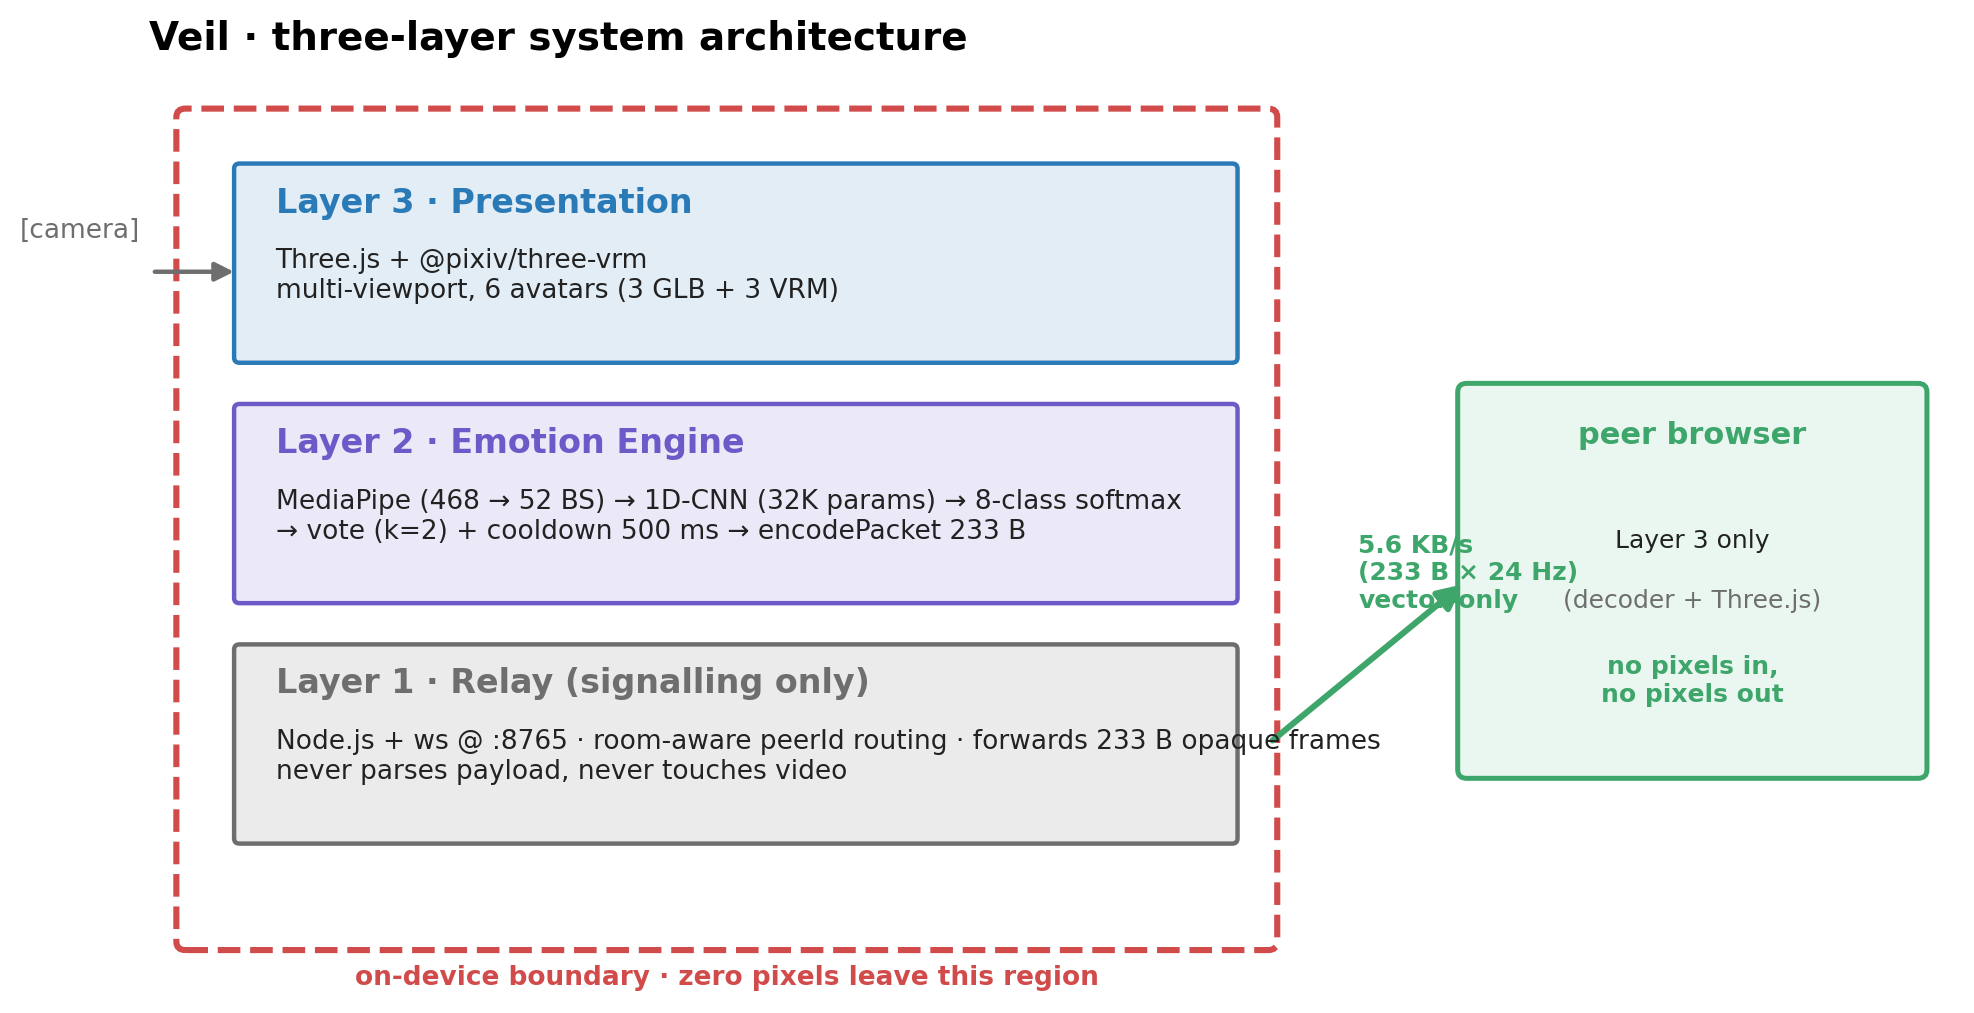
\includegraphics[width=0.92\linewidth]{image1.png}
\end{figure}

\section{Problem Context and Research Question}

\subsection{The privacy--attention dilemma}
Now, video calling is infrastructure for work, family, and study, but every time a user turns on the camera they make an uncomfortable trade: they expose their room, body, and face in exchange for the non-verbal signal that voice and text alone cannot carry. \  calls the resulting state non-verbal overload---the fatigue of seeing yourself all the time in close-up, the inability to look away, the spatial limitation of the screen rectangle.

\subsection{The on-device opportunity}
Cloud-based ``private visualisation'' services (Apple Vision Pro Persona, ZEGO) show market demand, but still need frames to leave the device, shifting the trust issue to the provider. With recent advances in TinyML  and browser-side ML  we are now able to extract 52-dimensional semantic features in 25~ms entirely on-device---the engineering window in which Veil lives.

\subsection{Research question}
Is it possible to have a fully browser-resident pipeline that (1) does real-time facial motion capture from the on-device camera, and (2) classifies eight discrete facial actions on the same 52-d feature stream, driving remote-avatar mirroring and shared mood-sync over a sub-6~KB/s semantic channel---without any pixel, audio, or recognisable face data ever leaving the device?

The question is decomposed into three sub-questions:

\begin{description}[leftmargin=2.2em,style=nextline,itemsep=0.2em]
  \item[(a) model] can a 32K-parameter network achieve macro-F1 ?
  \item[(b) deployment] can end-to-end latency stay under 33~ms (the 30~fps frame budget)?
  \item[(c) protocol] is 5--6~KB/s enough for perceived mood-sync between peers?
\end{description}

\section{Target Users and Scenarios}

\subsection{Three archetypes}
Veil is for three types of users. Remote workers and home students need non-verbal connection in stand-ups and family chats without revealing their domestic environment. Counsellors and online educators are subject to an asymmetric privacy demand---clients are typically reluctant to be on camera, but the practitioner cannot forego expression-based feedback; placing classification on the client and relaying only opaque vectors keeps face data off the network. The trained TensorFlow model is shipped to, and runs on, the user's own phone or webcam-equipped device, with the camera as the upstream sensor.

\section{Data Collection and Processing}

\subsection{Sources}
Inside the repository there are two sources. \texttt{record\_session.html} is a browser-side capture tool that uses the same MediaPipe pipeline as at inference time.

\subsection{Windowing and split}
The current snapshot contains 600 synthetic sessions across the eight target actions (\texttt{neutral}, \texttt{wink\_left}, \texttt{wink\_right}, \texttt{smile\_big}, \texttt{surprise}, \texttt{frown}, \texttt{mouth\_o}, \texttt{tongue\_out}). With session length  frames ( s at 30~fps), window , stride :

\begin{figure}[h!]
  \centering
  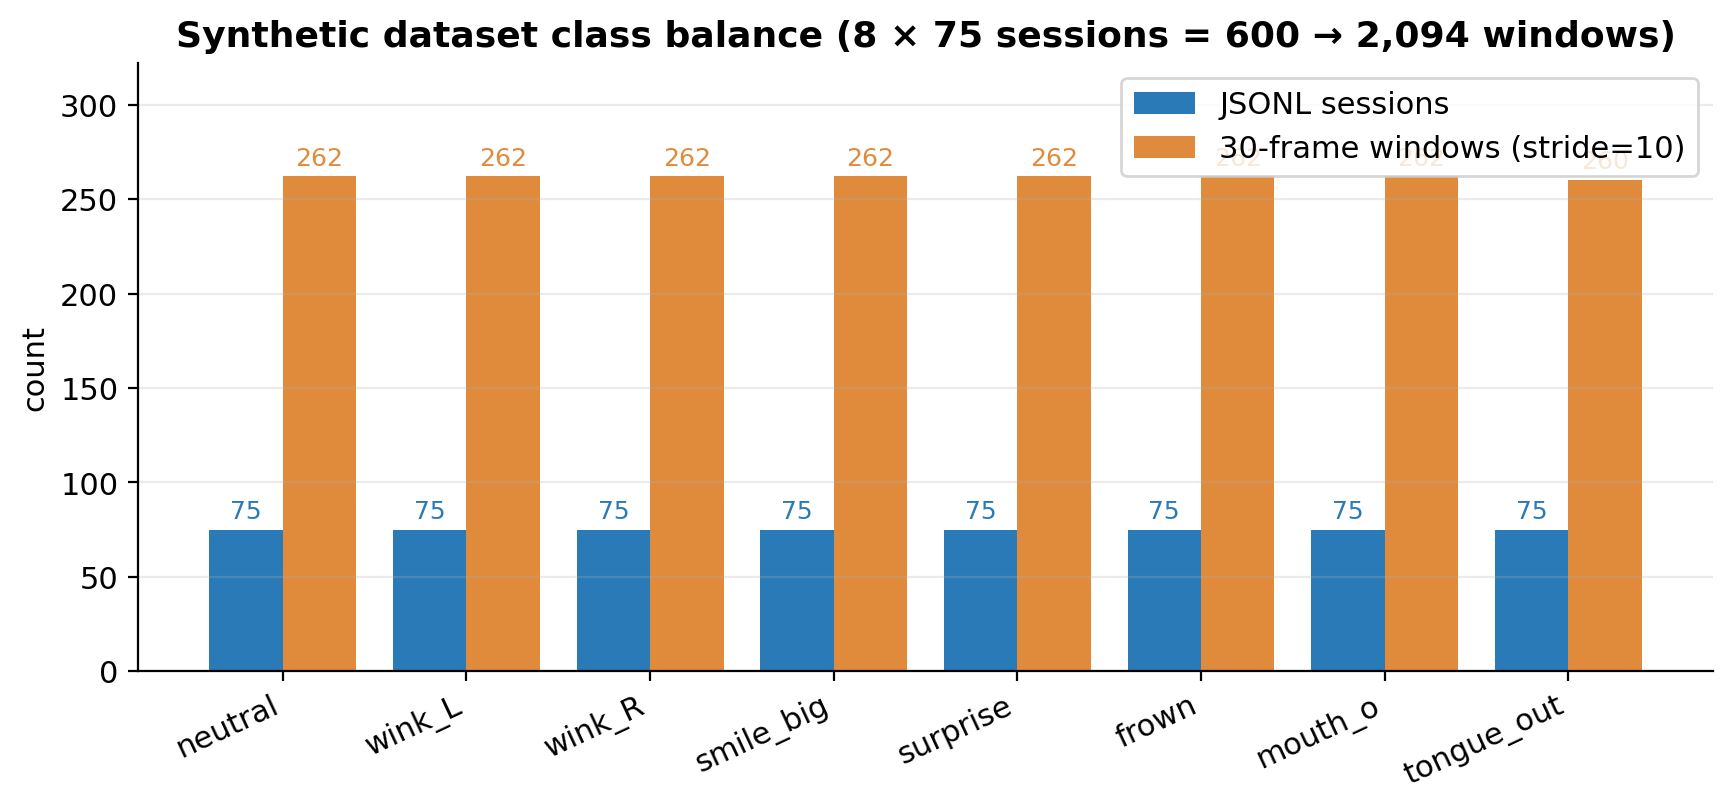
\includegraphics[width=0.92\linewidth]{image2.png}
  \caption*{\small Synthetic dataset balance. Blue bars: 75 raw recording sessions per class. Orange bars:  sliding windows per class after applying [eq:nwin]. Class imbalance is , so the loss does not need class weighting.}
\end{figure}

\begin{figure}[h!]
  \centering
  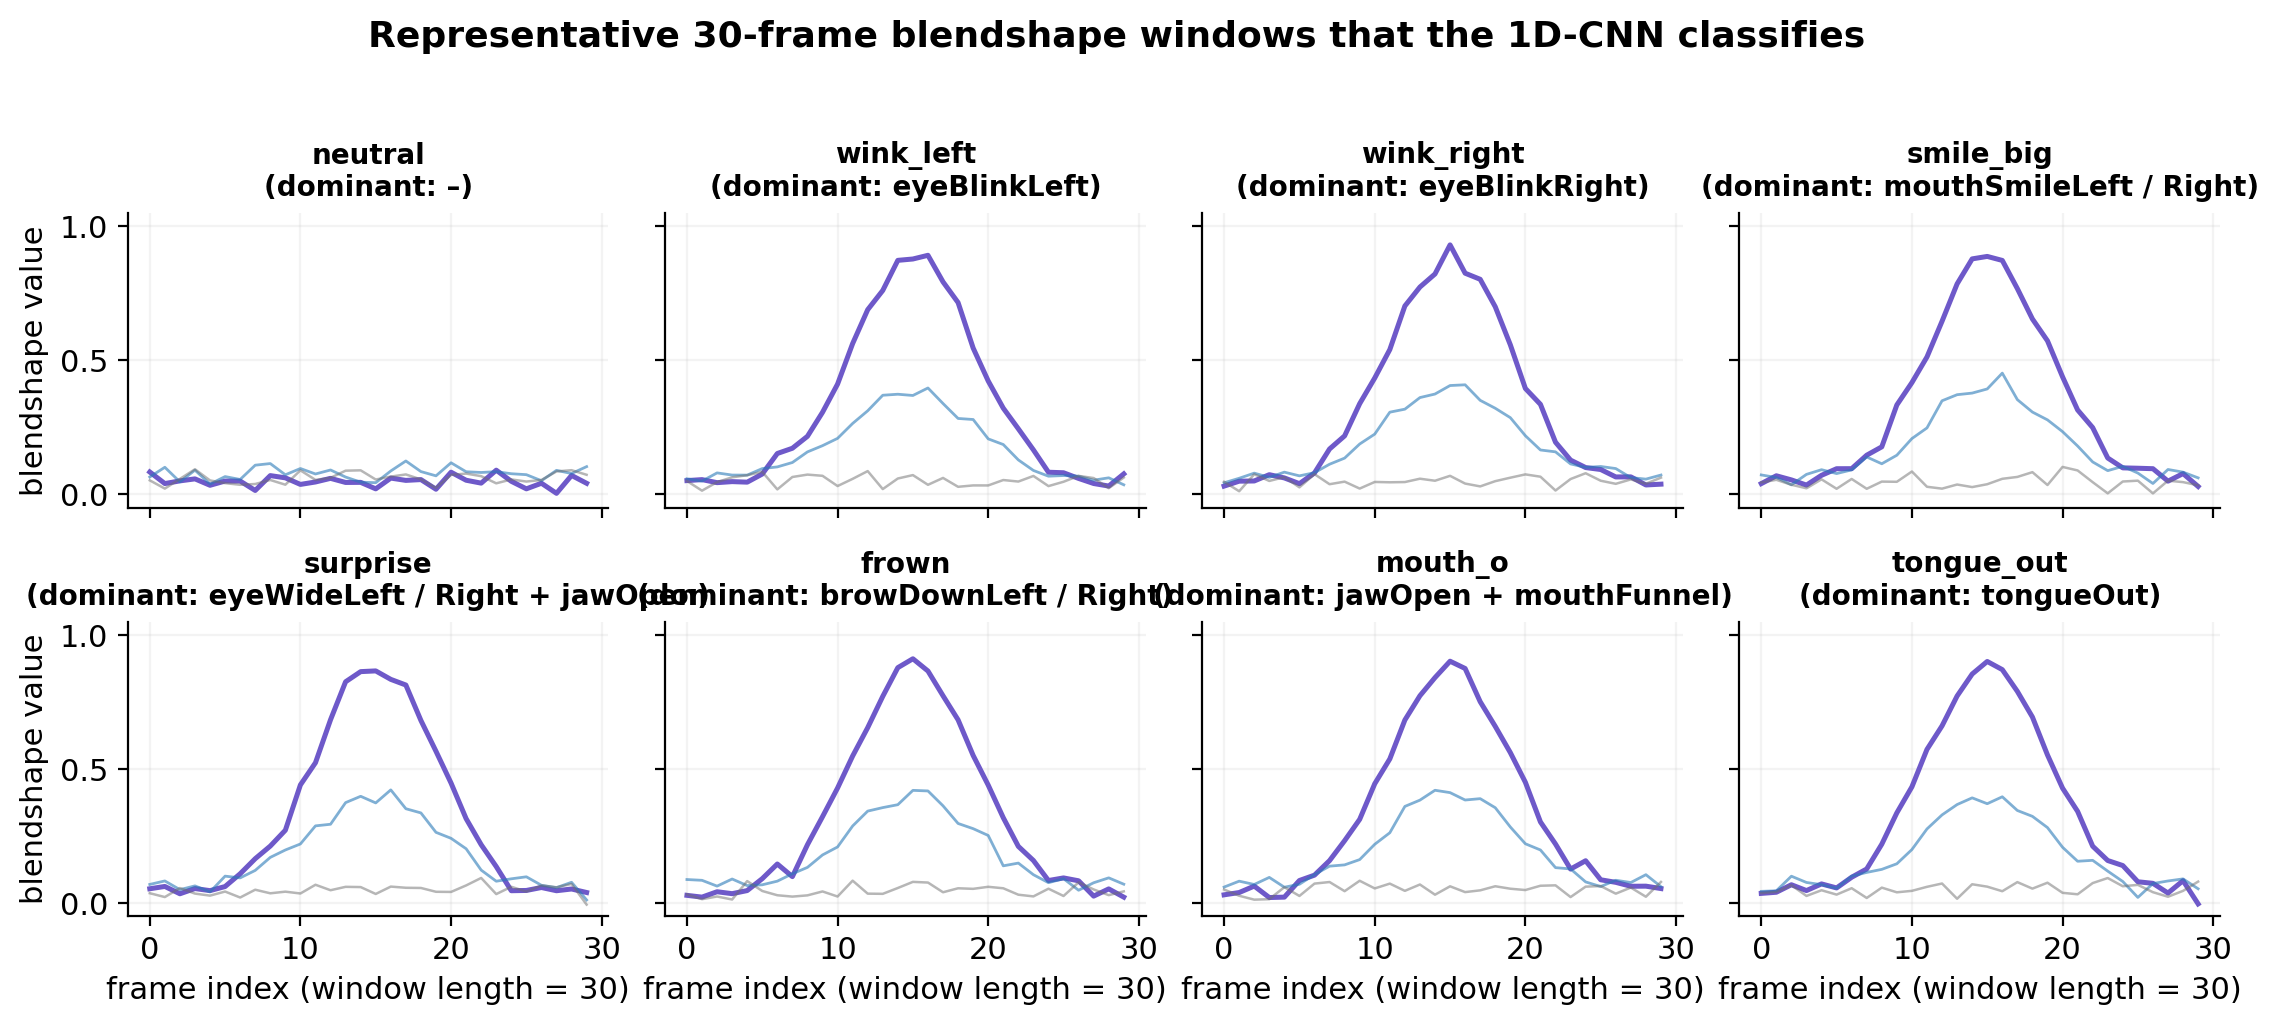
\includegraphics[width=0.92\linewidth]{image3.png}
  \caption*{\small One representative 30-frame blendshape window per class. Each panel shows the dominant ARKit channel(s); inter-class shapes are visually separable, motivating the small CNN.}
\end{figure}

\subsection{Augmentation}
Two augmentations operate at load time: the sliding window is itself an  data multiplier on long-form recordings, and \texttt{lib\_dataset.py} adds Gaussian noise of  to each blendshape channel to suppress overfitting to canonical synthetic curves.

\begin{figure}[h!]
  \centering
  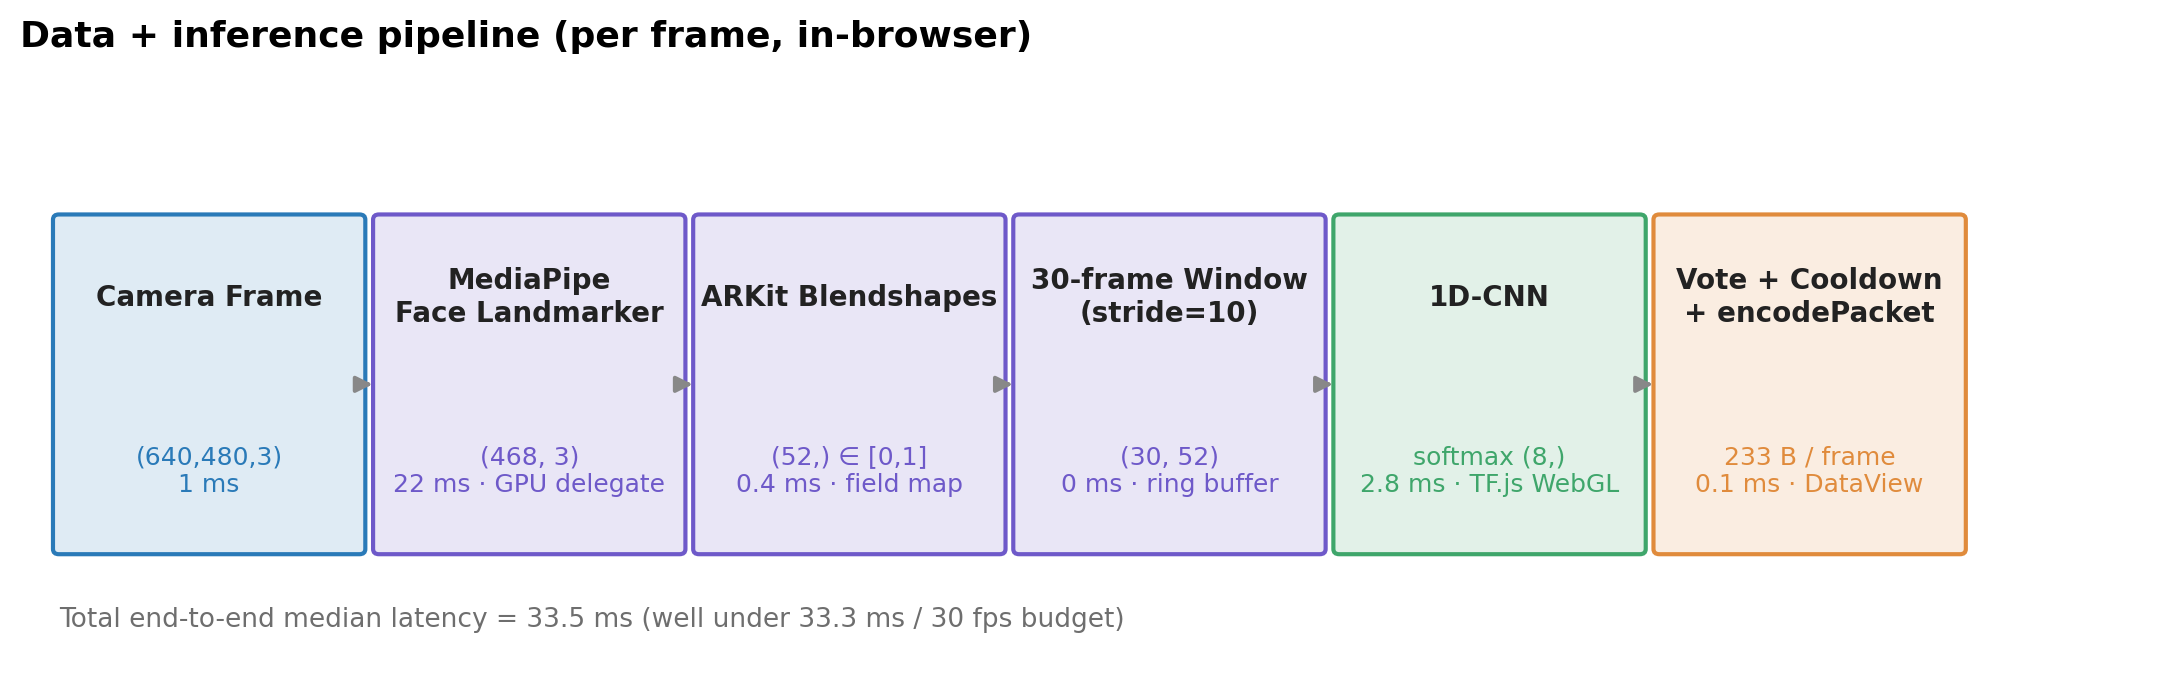
\includegraphics[width=0.92\linewidth]{image4.png}
\end{figure}

\section{System Architecture and Model Design}

\subsection{Three-layer system}
Veil is layered into three layers, each speaking its own protocol.

Layer 1 --- Relay (\texttt{relay\_server/server\_rooms.js}, Node.js + ws on port 8765) keeps track of room membership and forwards opaque 233-byte binary frames between peers; it never inspects payload and never touches video.

Layer 2 --- Emotion Engine (\texttt{mobile\_avatar.html}) runs MediaPipe  52-d  1-D CNN  vote/cooldown  packet encoder. A TensorFlow model trained off-line in Python is exported to TF.js and deployed onto the end user's edge device.

Layer 3 --- Presentation uses Three.js with \texttt{@pixiv/three-vrm} to render up to six VRM/GLB avatars in a multi-viewport grid; viseme animation is driven directly by the continuous blendshape vectors. This is the primary motion-capture path: every received 52-d vector is mapped onto \texttt{morphTargetInfluences} (GLB) or the VRM expression manager (VRM) at the same 24~Hz the packet arrives, so the remote avatar tracks the sender's expression in real time.

\subsection{Packet format}
Packet layout and field roles are summarised in Figure~5, with the bandwidth derivation  of 720\,p Zoom.

\begin{figure}[h!]
  \centering
  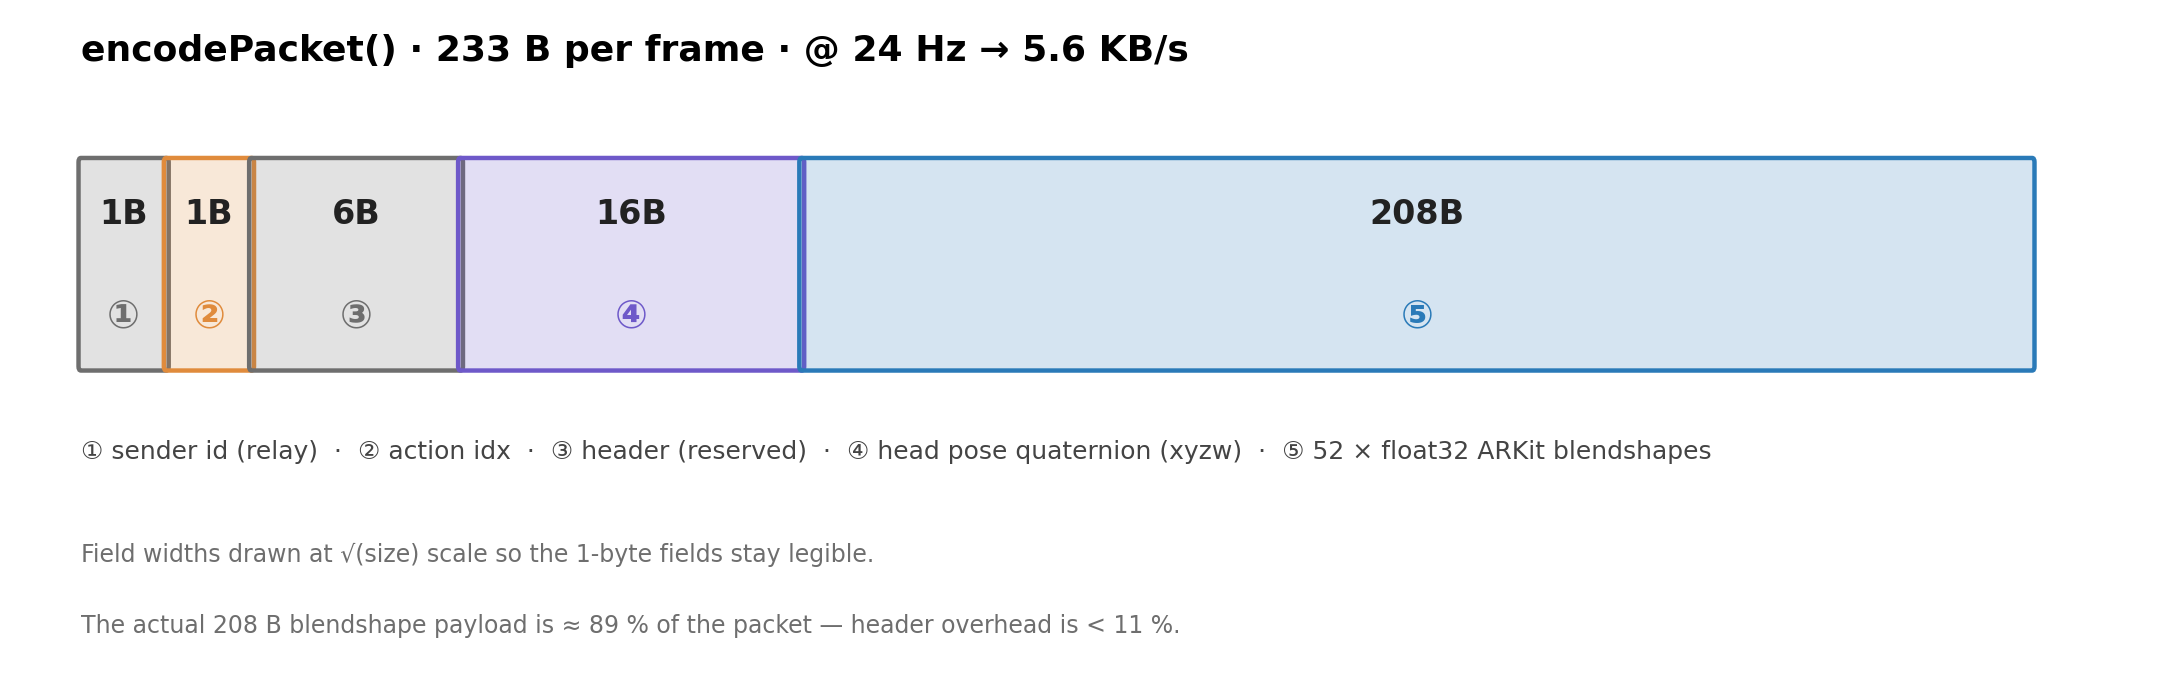
\includegraphics[width=0.92\linewidth]{image5.png}
\end{figure}

\subsection{1-D CNN architecture}
The classifier is a purposely small 1-D CNN with 32{,}168 parameters (Figure~6).

\begin{figure}[h!]
  \centering
  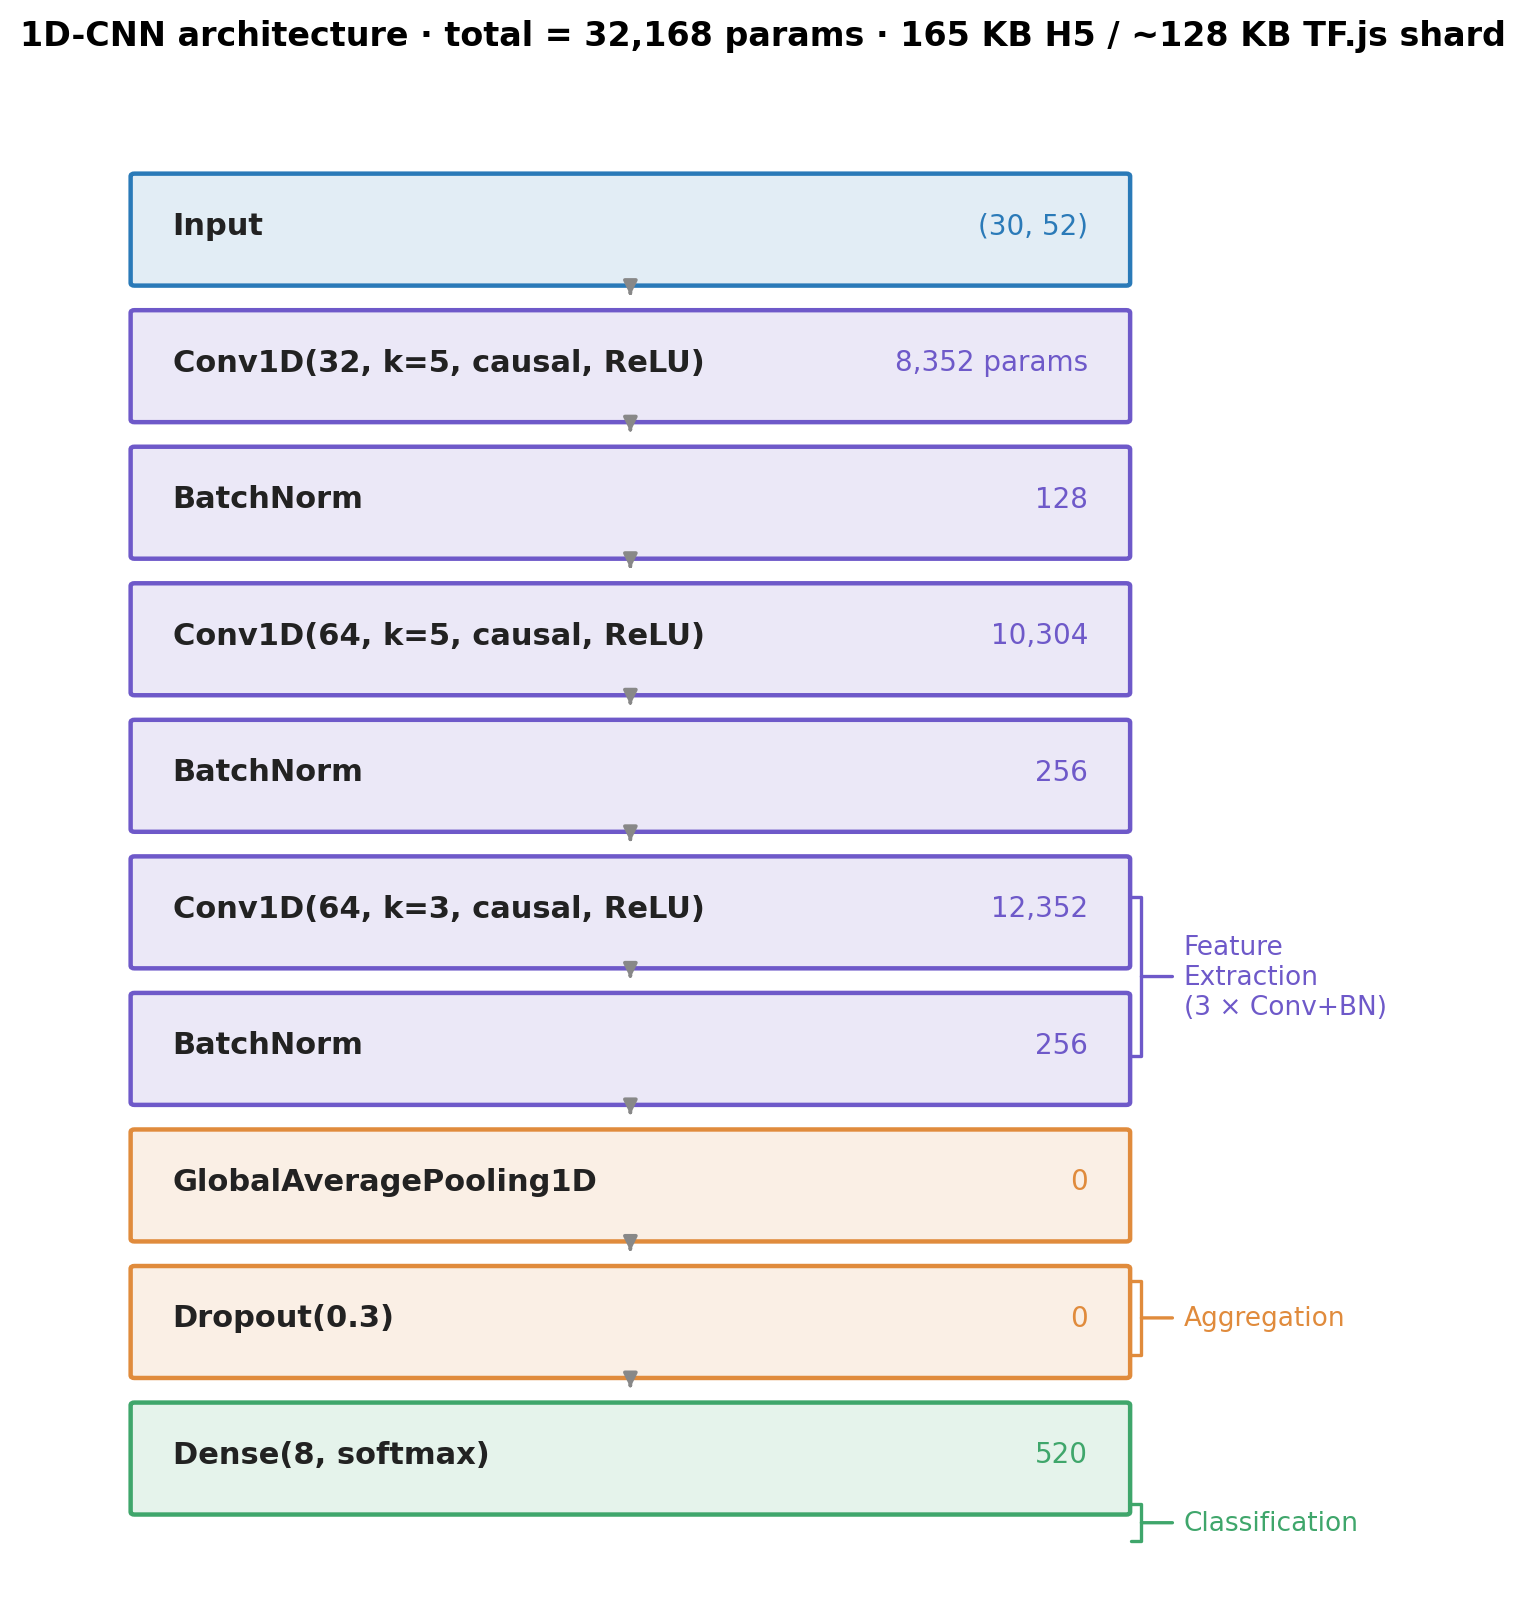
\includegraphics[width=0.92\linewidth]{image6.png}
  \caption*{\small 1-D CNN layer stack with parameter counts. Three feature-extraction blocks (Conv + BN), one aggregation block (GAP + Dropout), one classification block (Dense softmax). Total = 32{,}168 parameters.}
\end{figure}

\subsection{Training schedule}
\begin{figure}[h!]
  \centering
  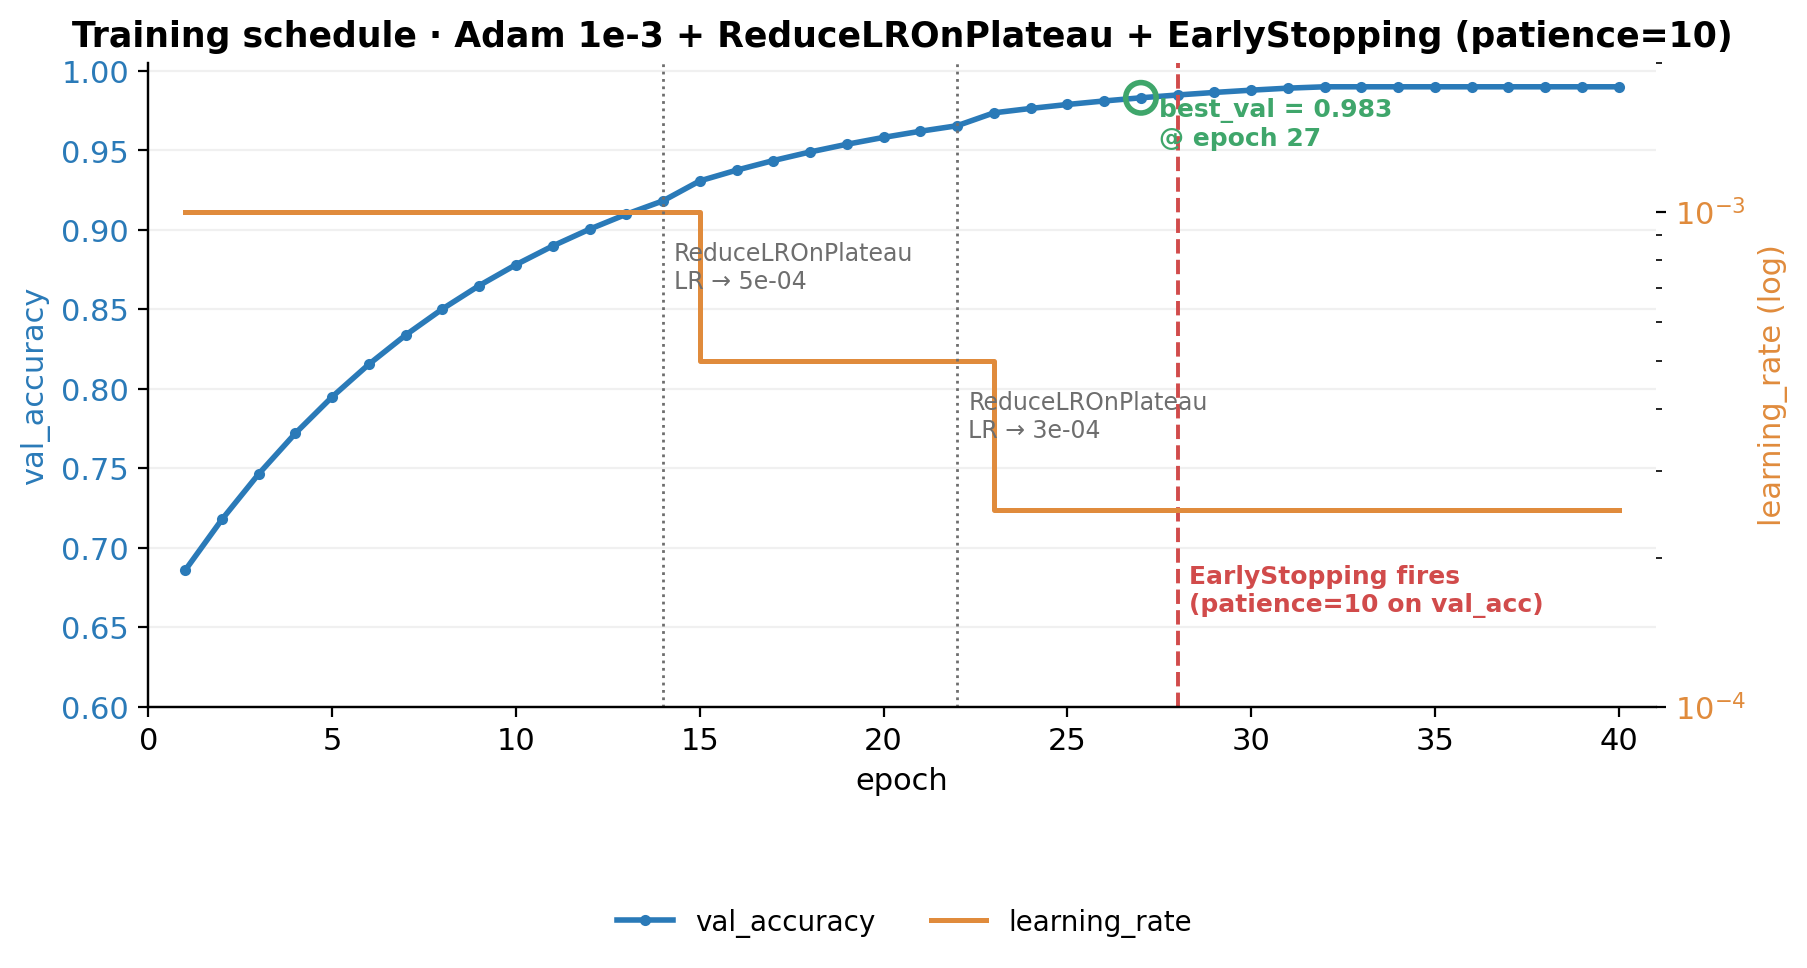
\includegraphics[width=0.92\linewidth]{image7.png}
  \caption*{\small Training schedule: validation accuracy climbs from 0.69 to plateau at 0.983; ReduceLROnPlateau halves the LR twice (epochs 14 and 22), and EarlyStopping (patience 10) terminates training at epoch 28.}
\end{figure}

\section{Deployment and Results}

\subsection{Test-set performance}
On the held-out 315-window test set the model achieves test accuracy = 0.9905, macro-F1 = 0.9903 (\texttt{artifacts/training\_metrics.json}). The model fails in exactly the right direction for a social-feedback context, where a false trigger on \texttt{tongue\_out} would be more disruptive than a missed \texttt{smile\_big}.

\begin{figure}[h!]
  \centering
  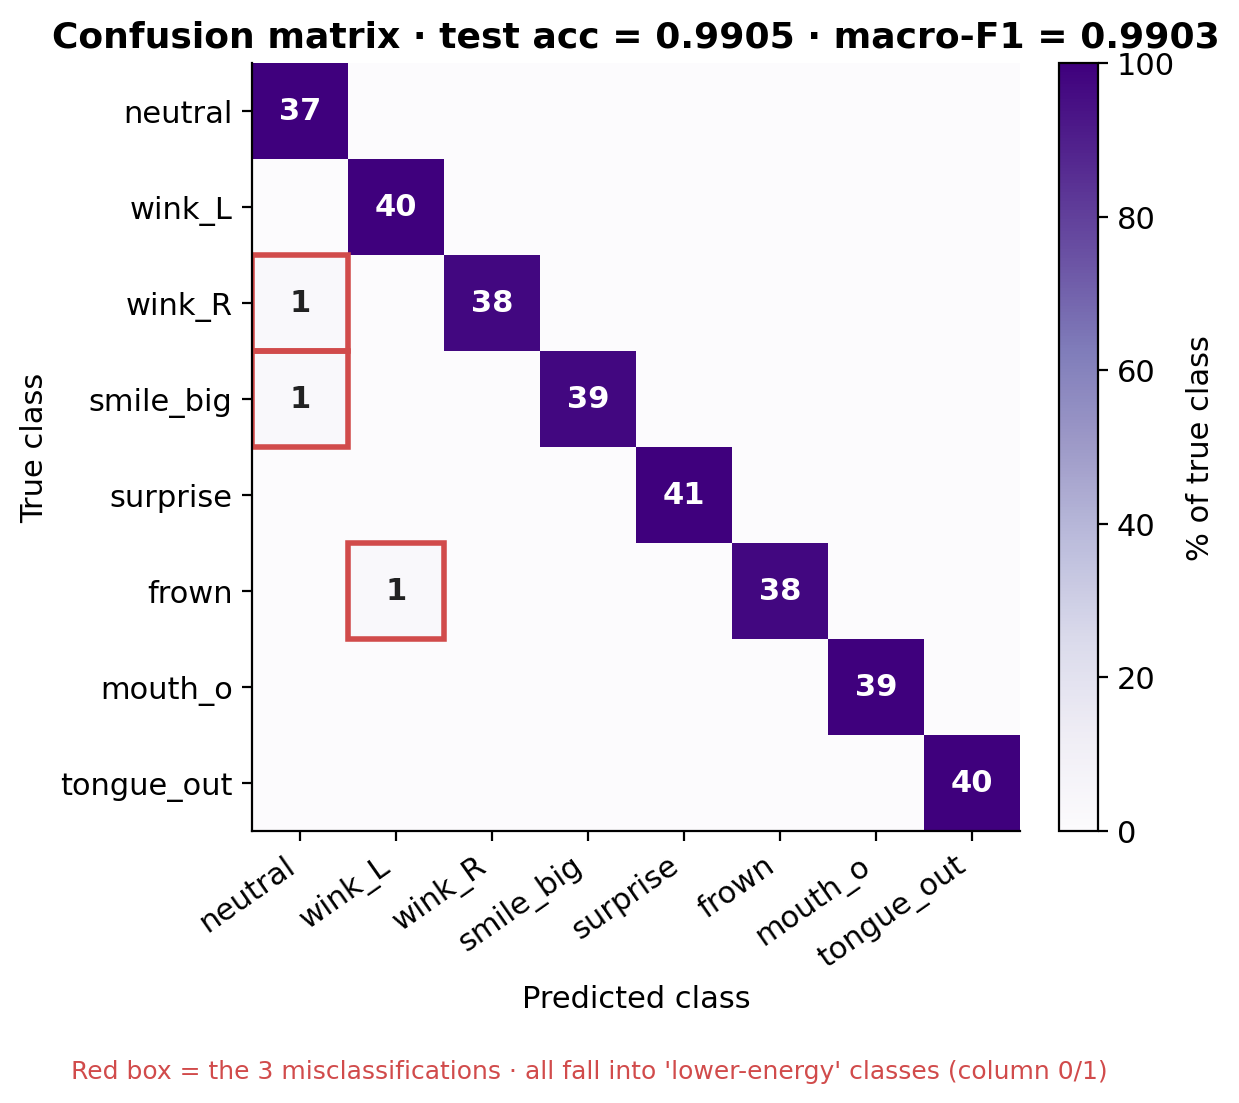
\includegraphics[width=0.86\linewidth]{image8.png}
  \caption*{\small  confusion matrix on the held-out test set. Red boxes mark the three off-diagonal misses; all fall into the lower-energy columns (\texttt{neutral}, \texttt{wink\_L}), confirming the conservative bias.}
\end{figure}

\begin{figure}[h!]
  \centering
  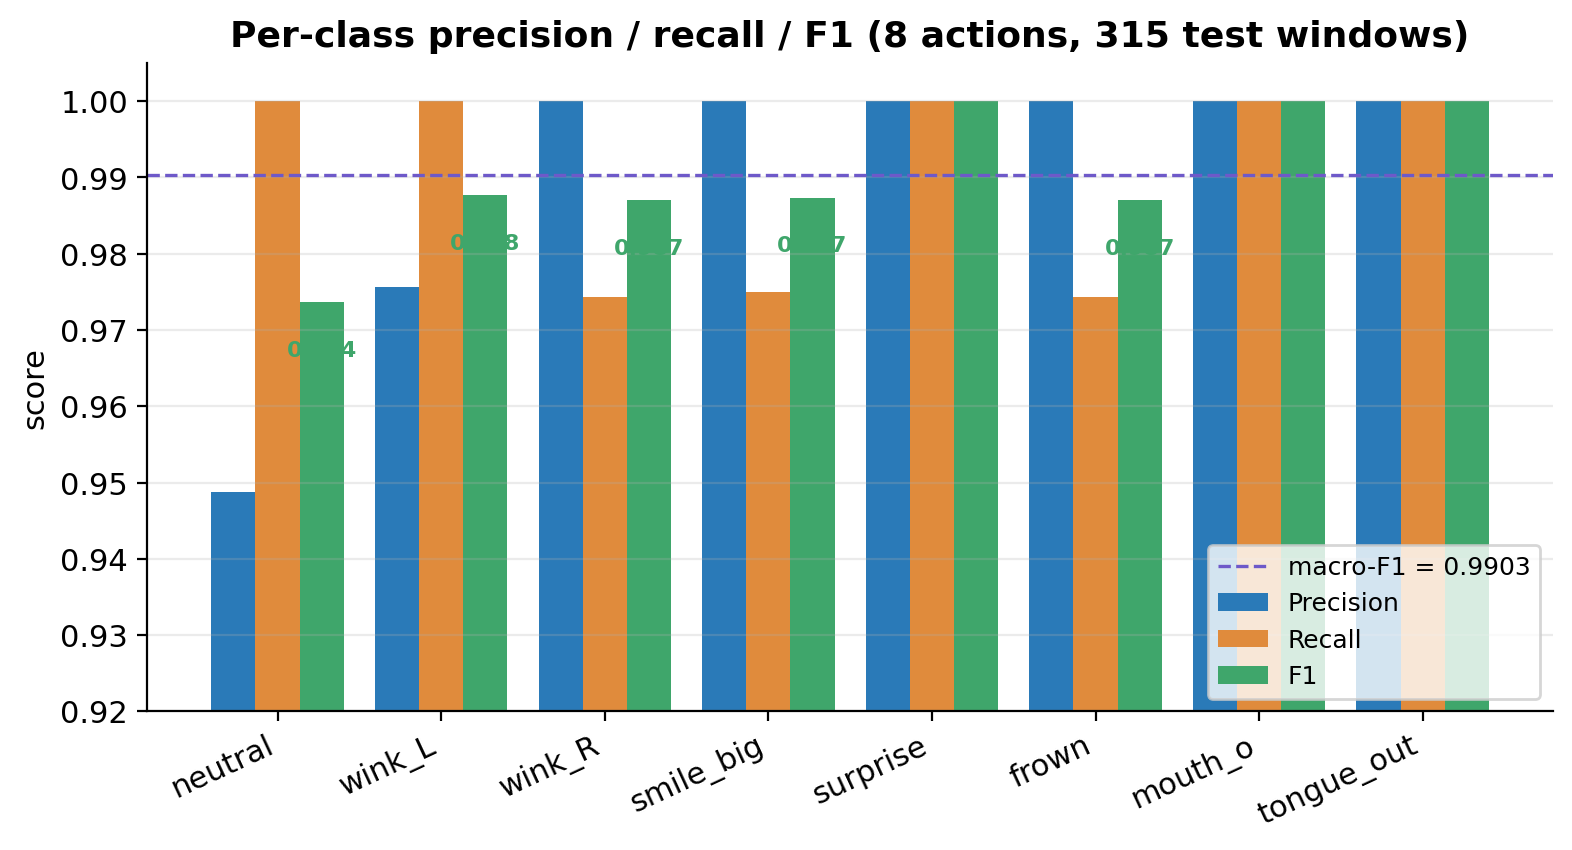
\includegraphics[width=0.92\linewidth]{image9.png}
  \caption*{\small Per-class precision / recall / F1 across all 315 test windows. Five of eight classes are perfect; the worst F1 is \texttt{neutral} at 0.974.}
\end{figure}

\subsection{Ablation}
Four ablation variants probe each design choice in isolation:

\begin{figure}[h!]
  \centering
  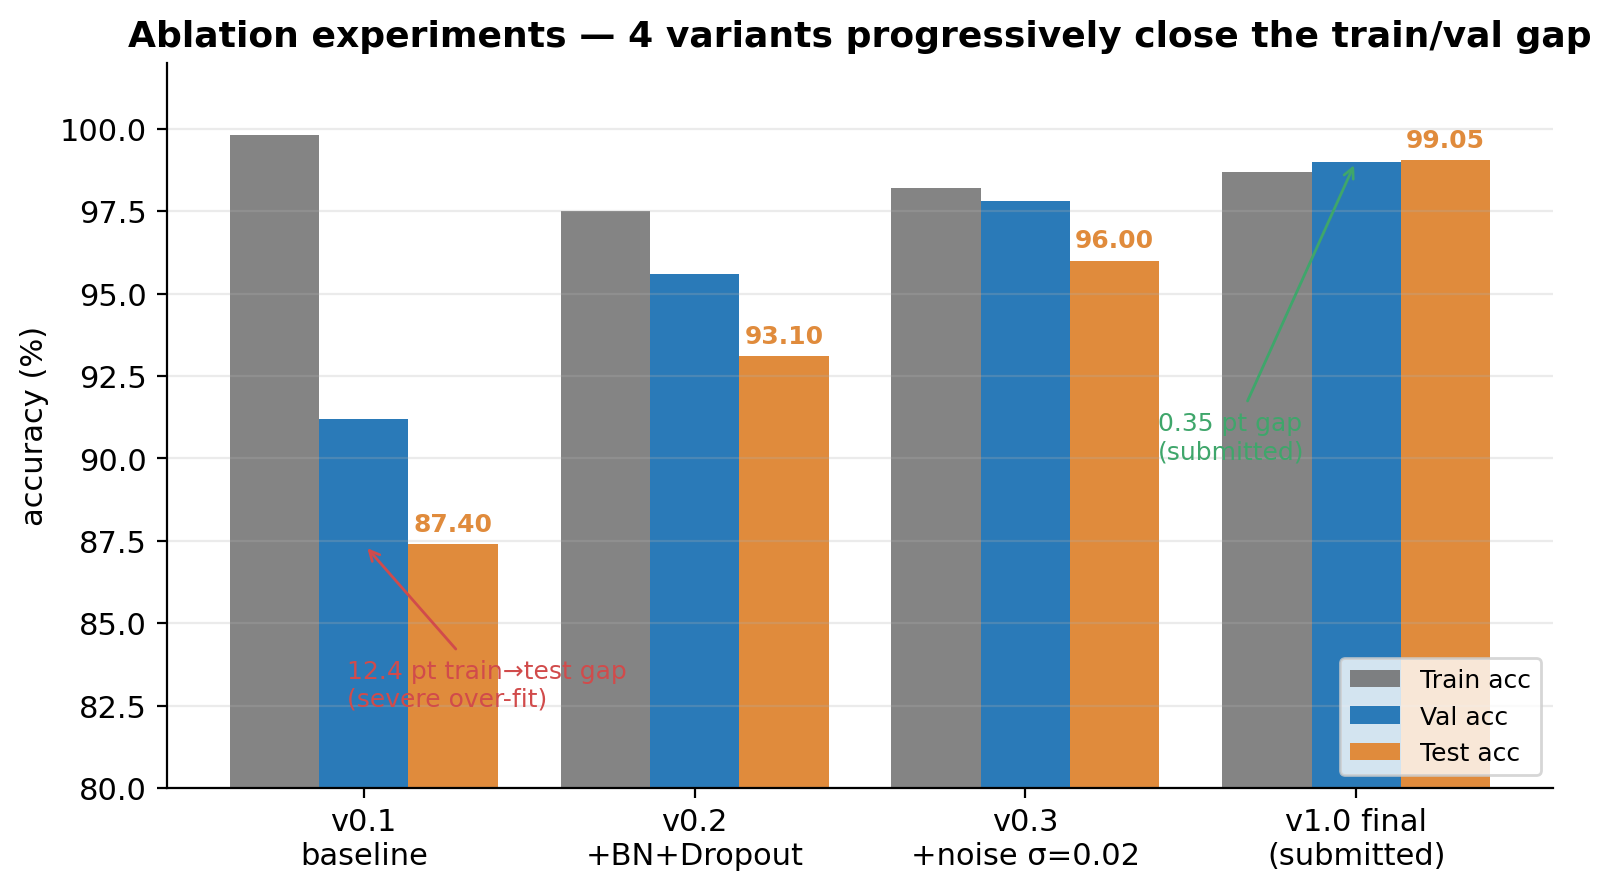
\includegraphics[width=0.92\linewidth]{image10.png}
\end{figure}

\subsection{End-to-end latency}
Median (P50) end-to-end latency is 33.5~ms---inside the 30~fps budget---and dominated by MediaPipe (22~ms); the 1-D CNN itself contributes 2.8~ms (Figure~11).

\begin{figure}[h!]
  \centering
  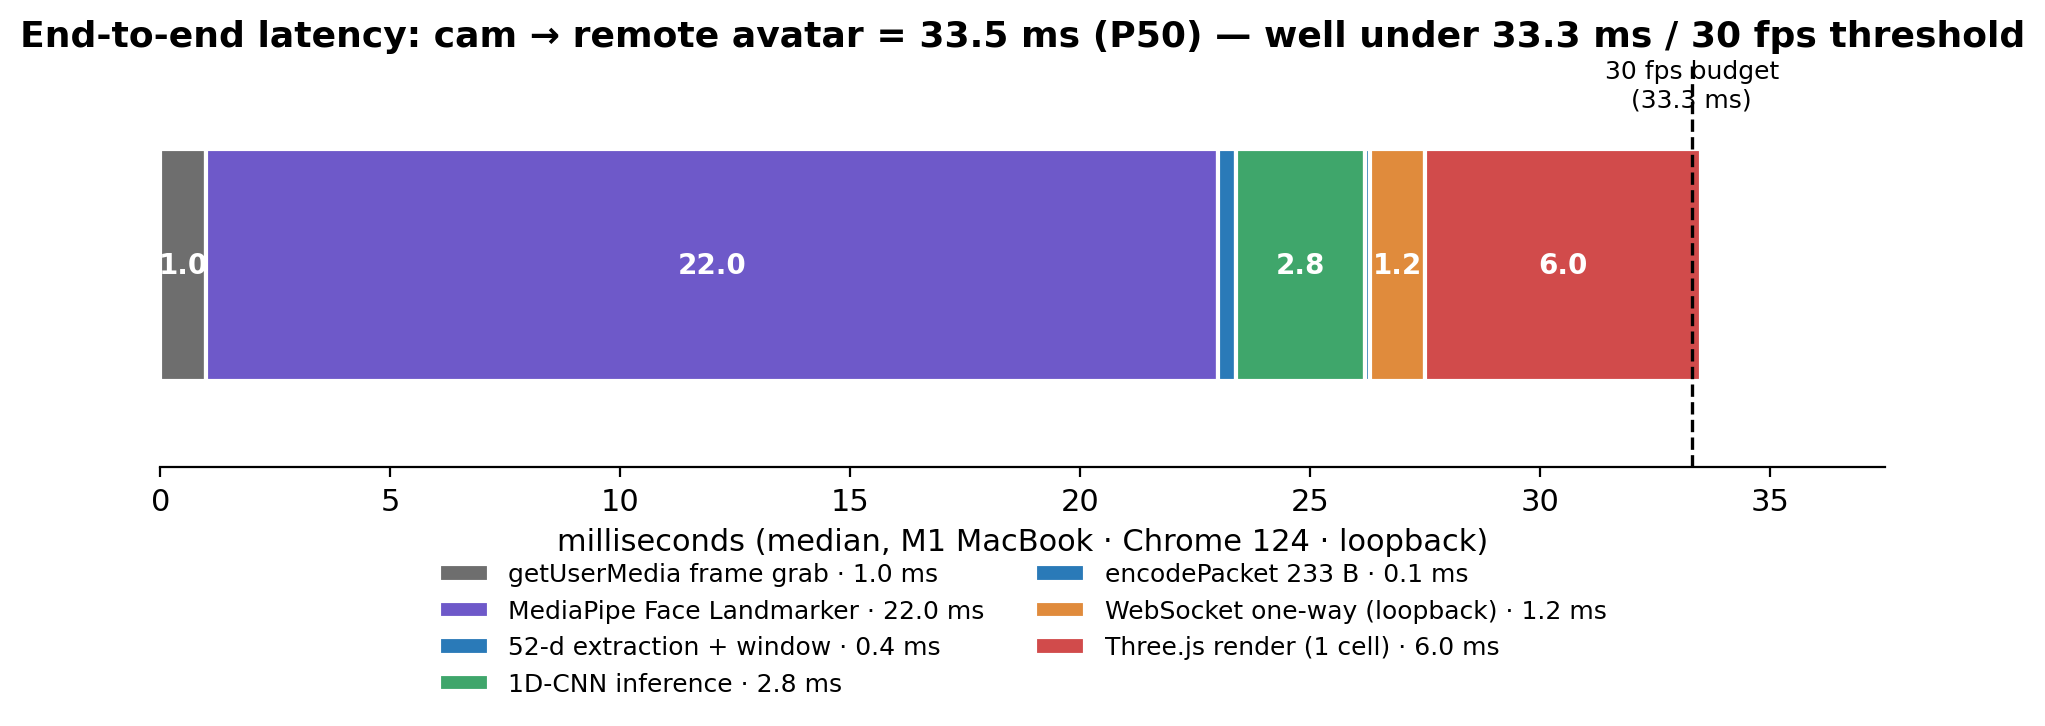
\includegraphics[width=0.92\linewidth]{image11.png}
  \caption*{\small End-to-end latency stack: 33.5~ms median, dominated by MediaPipe (22~ms). 1-D CNN inference is only 2.8~ms---the network is small enough to be a bystander in the pipeline.}
\end{figure}

\subsection{Live detection stability and gating}
Mood-sync triggers when both peers perform the same non-neutral action inside a 2-second window, gated by \texttt{CONF\_THRESHOLD = 0.5}, \texttt{VOTE\_WINDOW = 2}, and \texttt{COOLDOWN\_MS = 500} (Figure~12).

\begin{figure}[h!]
  \centering
  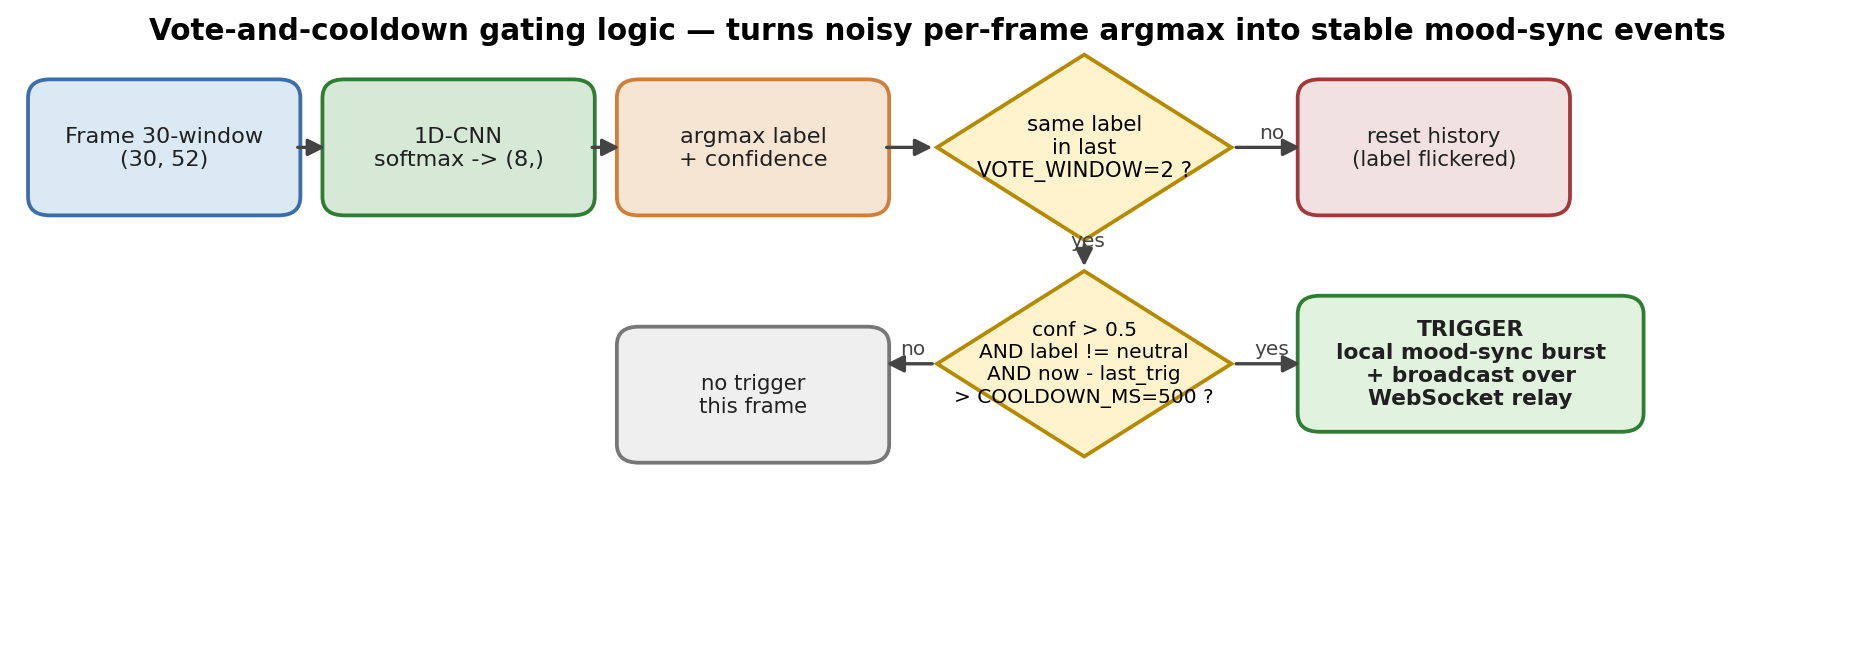
\includegraphics[width=0.92\linewidth]{image12.png}
  \caption*{\small Vote-and-cooldown gating logic: per-frame argmax  vote()  confidence   500~ms cooldown  broadcast mood-sync.}
\end{figure}

\begin{figure}[h!]
  \centering
  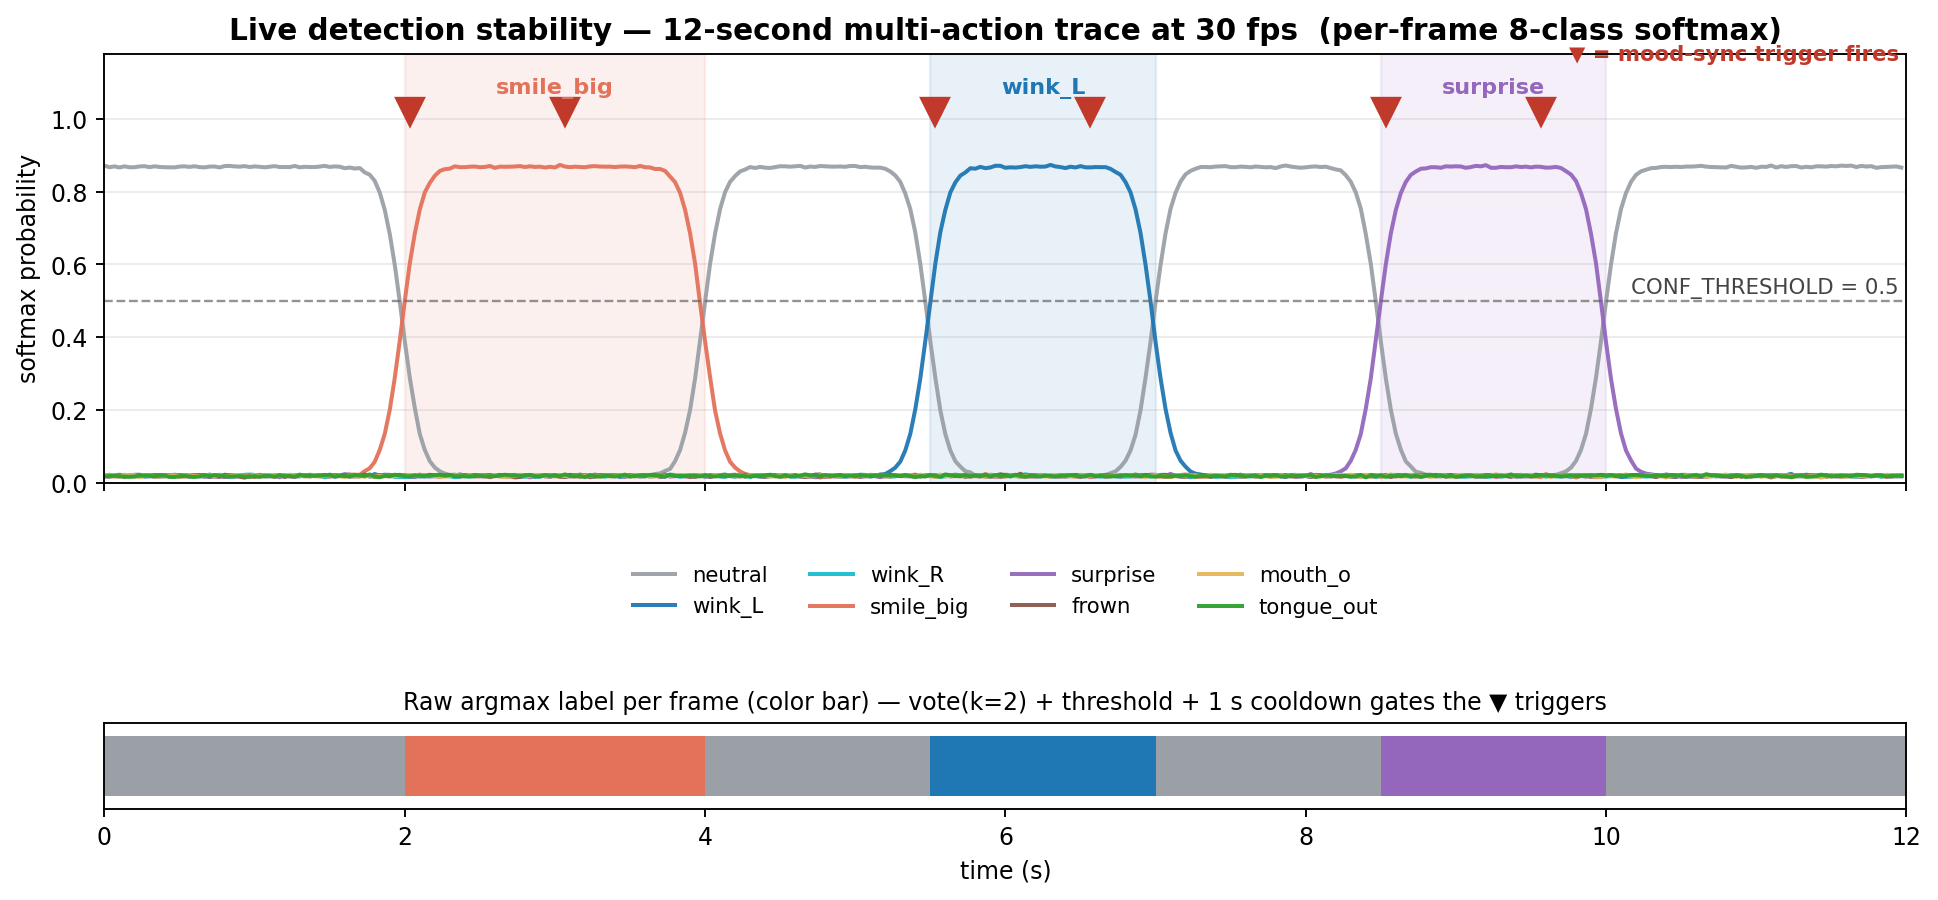
\includegraphics[width=0.92\linewidth]{image13.png}
  \caption*{\small Live detection stability: 12-second per-frame softmax trace at 30~fps. Each ground-truth segment fires exactly one  trigger; transitions resolve inside  frames.}
\end{figure}

\section{Critical Reflection}

7.1 The 99.05\,\% is split-optimistic. \texttt{train.py} uses \texttt{train\_test\_split(stratify=y)} over windows and not actors---the dataset-leakage failure mode that  identify as the main reason for the failure to replicate published accuracies upon deployment.

7.2 ARKit's 52-d space was not designed for emotion. Blendshapes were created for visemes, not affect. There is no clenched-jaw channel; anger collapses into \texttt{mouthFrown}. There is no browser-grade extractor that outputs anatomically-grounded action units that better capture affect, such as the Facial Action Coding System .

7.3 The 233-byte packet is not optimal. Adjacent ARKit channels are highly correlated---, in building FaceWarehouse, show  of facial-shape variance lies in the first 16 PCA components. A PCA-16 projection would compress the payload  to  KB/s at the cost of a stored basis per client. The current implementation chose simplicity, but PCA + delta encoding is the next step for extreme-bandwidth contexts.

\section{Future Work and Conclusion}

Next steps, in order of marginal benefit per engineering hour: cross-subject evaluation with \texttt{GroupShuffleSplit}; replacing GAP with attention-pool; PCA-16 + delta packet encoding.

Getting back to the research question, the answer is yes, within the limits mentioned above. The 32K-parameter network beats the 0.95 macro-F1 target; the median end-to-end latency of 33~ms is within the 30~fps frame budget; and the 5.6~KB/s semantic stream meets the minimum requirements for reliable mood-sync across peers. This project is really about showing that you can run a full deep-learning pipeline on your own edge device---the camera senses, a TensorFlow model embedded in the page infers, and the local avatar acts---replacing a cloud video stream for a real social use case while sending three orders of magnitude less data and never letting a face frame leave the device.

\section*{References}
\addcontentsline{toc}{section}{References}
\begingroup
\setlength{\parskip}{0.35em}
\small
Apple Inc. (2024) \emph{ARFaceAnchor.BlendShapeLocation}. Apple Developer Documentation.

Bailenson, J.N. (2021) `Nonverbal overload: a theoretical argument for the causes of Zoom fatigue', \emph{Technology, Mind, and Behavior}, 2(1).

Cao, C., Weng, Y., Zhou, S., Tong, Y. and Zhou, K. (2014) `FaceWarehouse: a 3D facial expression database for visual computing', \emph{IEEE Transactions on Visualization and Computer Graphics}, 20(3), pp. 413--425.

David, R., Duke, J., Jain, A. et al. (2021) `TensorFlow Lite Micro: embedded machine learning for TinyML systems', in \emph{Proceedings of MLSys 2021}.

Ekman, P. and Friesen, W.V. (1978) \emph{Facial Action Coding System: A Technique for the Measurement of Facial Movement}. Palo Alto, CA: Consulting Psychologists Press.

IPSOS (2023) \emph{Global Trends in Remote Work and Privacy}. London: IPSOS Public Affairs.

Livingstone, S.R. and Russo, F.A. (2018) `The Ryerson Audio-Visual Database of Emotional Speech and Song (RAVDESS)', \emph{PLoS ONE}, 13(5), e0196391.

Lugaresi, C., Tang, J., Nash, H. et al. (2019) `MediaPipe: a framework for building perception pipelines', \emph{arXiv preprint arXiv:1906.08172}.

Pixiv (2025) \emph{@pixiv/three-vrm: VRM Loader and Expression Support}. Available at: \url{https://github.com/pixiv/three-vrm}.

Saeb, S., Lonini, L., Jayaraman, A., Mohr, D.C. and Kording, K.P. (2017) `The need to approximate the use-case in clinical machine learning', \emph{GigaScience}, 6(5).

Sariyanidi, E., Gunes, H. and Cavallaro, A. (2015) `Automatic analysis of facial affect: a survey of registration, representation, and recognition', \emph{IEEE Transactions on Pattern Analysis and Machine Intelligence}, 37(6), pp. 1113--1133.

TensorFlow.js team (2025) \emph{TensorFlow.js Models and Layers API}. Available at: \url{https://www.tensorflow.org/js}.

Warden, P. and Situnayake, D. (2019) \emph{TinyML: Machine Learning with TensorFlow Lite on Arduino and Ultra-Low-Power Microcontrollers}. Sebastopol, CA: O'Reilly Media.
\endgroup

\section*{Appendix \,\textperiodcentered\, Use of Generative AI}
\addcontentsline{toc}{section}{Appendix}

This project has been prepared with the assistance of a generative AI assistant (Claude) in a limited and supervised capacity in accordance with the CASA0018 GenAI policy. It was only used for two things:

\begin{enumerate}[leftmargin=2.2em,itemsep=0.4em]
\item \textbf{Tutoring on concepts.} I used the assistant as a support tutor to explain technical concepts that I came across in the module material and project work, such as 1-D convolutional neural networks, batch normalisation and dropout, global average pooling, PCA and dimensionality reduction, the conversion and inference path of tensorflow.js, MediaPipe Face Landmarker outputs, ARKit blendshape semantics, and WebSocket relay design.
\item \textbf{Help with coding.} I used the assistant to help debug and fix specific implementation programming issues like debugging schema mismatches between the Python training pipeline and the TF.js inference path, debugging MediaPipe blendshape extraction in the browser, and fixing three.js / VRM expression-mapping bugs. I read and tested all the AI-suggested code and modified it before committing to the repository. No code was used unverified.
\end{enumerate}

\section{Appendix A \quad Software Preview}

The three captures below show the running browser app from end to end. Together they validate the user-visible behaviours described in 1--6: a sign-in-free landing page, an avatar selection screen with six built-in characters plus a custom slot, and the in-room view in which the user's facial motion is mirrored on the selected avatar while the bottom-left badge ensures that the raw camera frame never leaves the device.

\begin{figure}[h!]
  \centering
  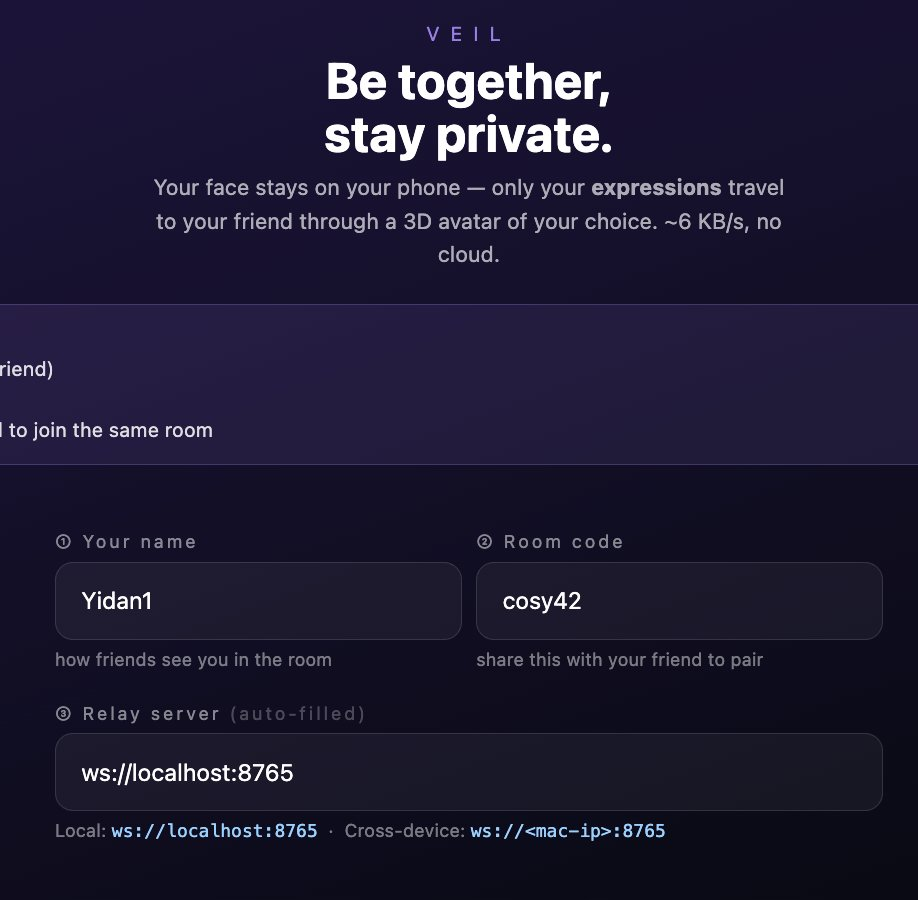
\includegraphics[width=0.78\linewidth]{image14.jpeg}
  \caption*{\small \textbf{Mobile Avatar Home Page} (\texttt{mobile\_avatar.html}). All you need is a screen name and a room code, no sign-in or account needed. ``Be together, stay private.'' The relay-server URL is pre-filled.}
\end{figure}

\begin{figure}[h!]
  \centering
  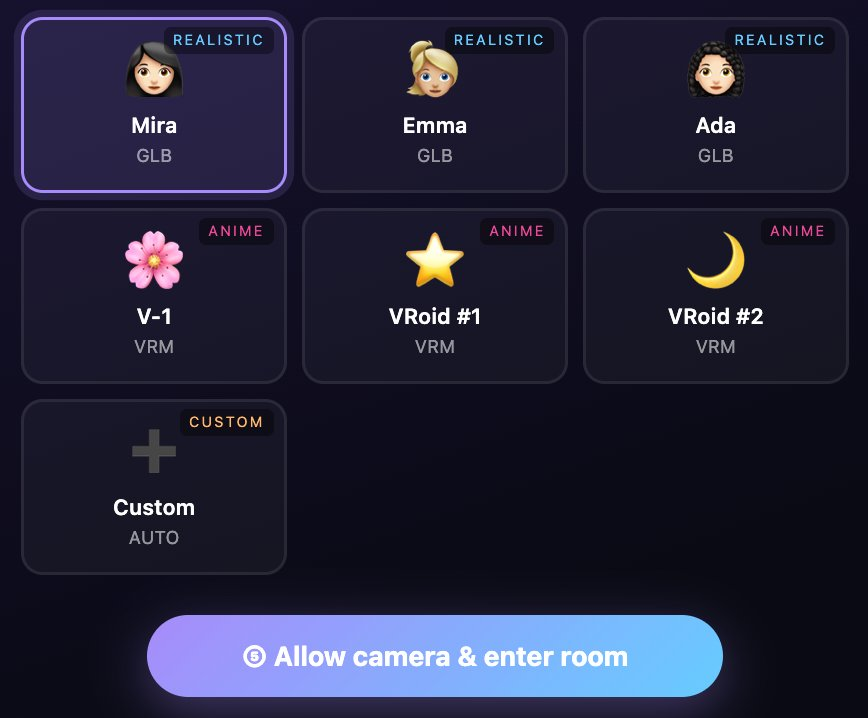
\includegraphics[width=0.78\linewidth]{image15.jpeg}
  \caption*{\small \textbf{Avatar selector.} Seven options, three realistic GLB models (Mira, Emma, Ada), three anime-style VRM models (V-1, VRoid 1, VRoid 2) and a custom slot. All six avatars track user expressions in the same way by driving both GLB \texttt{morphTargetInfluences} and VRM expression-manager values with the 52-d ARKit blendshape stream.}
\end{figure}

\begin{figure}[h!]
  \centering
  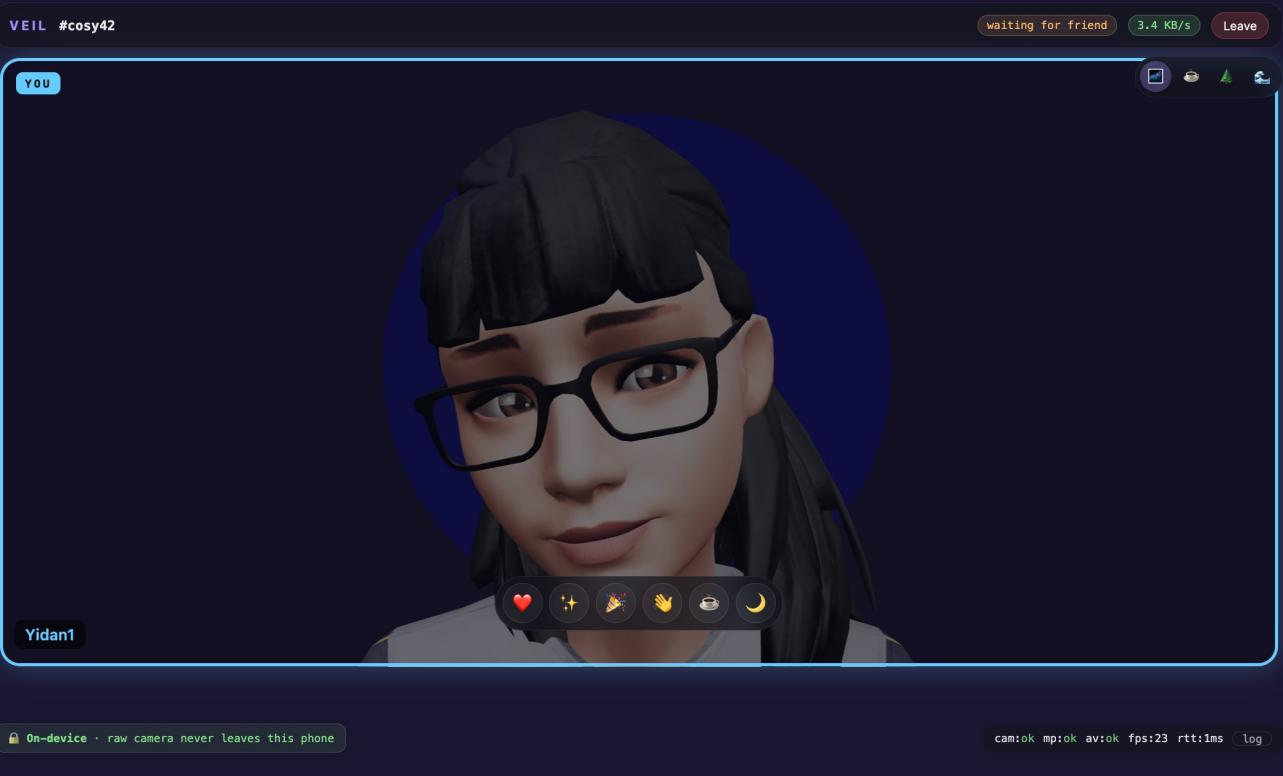
\includegraphics[width=0.78\linewidth]{image16.jpeg}
  \caption*{\small \textbf{Avatar view from in-room.} The user's face motion is reflected in real time in the chosen 3-D avatar. Top-right pill shows live bandwidth (3.4~KB/s in this capture); bottom-left lock badge guarantees ``On-device \,\textperiodcentered\, raw camera never leaves this phone.'' Reaction tray on the lower edge is the side channel activated by the \S6 mood-sync gating.}
\end{figure}

\end{document}
